\section{Signal model}
%Describe Fan's signal model 
(Fan, in progress) This section describes a MiniBooNE eLEE model used as a tool to benchmark compatibility of MicroBooNE's data with a possible $\nu_e$ low energy excess. This model is constructed using MiniBooNE dataset from its 2020 result \cite{MiniBooNEpaper}, where the observation of LEE is shown in Fig.~\ref{fig:MBLEE}. 

\begin{figure}[H]
    \centering
    \begin{subfigure}{0.52\linewidth}
        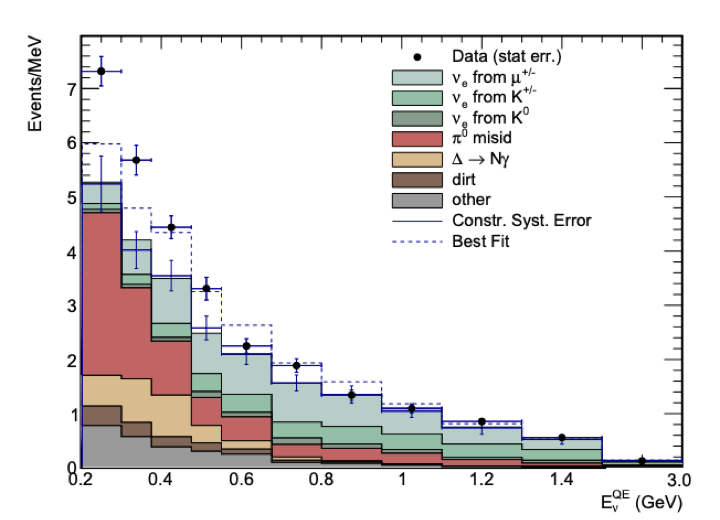
\includegraphics[width=\linewidth]{technote/SignalModel/Figures/MB CCQE.png}
        \caption{MiniBooNE CCQE neutrino energy distributions, in 200 $< E_{\nu}^{\rm{CCQE}} <$ 3000 MeV energy range.}
    \end{subfigure}
    \begin{subfigure}{0.49\linewidth}
        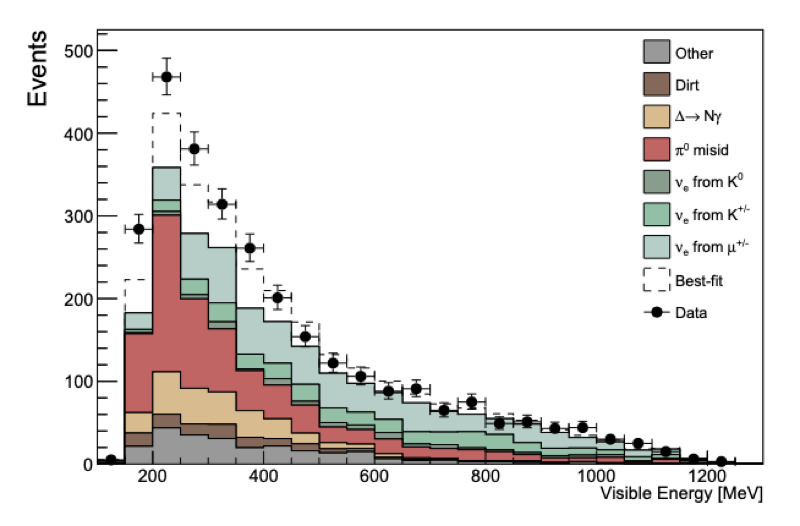
\includegraphics[width=\linewidth]{technote/SignalModel/Figures/MB ShwKE.png}
        \caption{MiniBooNE shower energy distributions, in 200 $< E_{\nu}^{\rm{CCQE}} <$ 1250 MeV energy range.}
    \end{subfigure}    
    \begin{subfigure}{0.49\linewidth}
        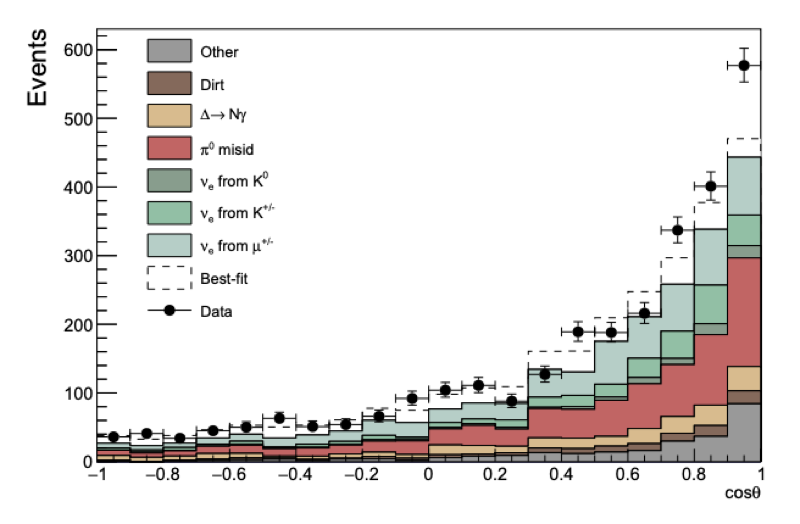
\includegraphics[width=\linewidth]{technote/SignalModel/Figures/MB ShwAngle.png}
        \caption{MiniBooNE shower $\cos\theta$ distributions, in 200 $< E_{\nu}^{\rm{CCQE}} <$ 1250 MeV energy range.}
    \end{subfigure}
    \caption{MiniBooNE low energy excess in CCQE neutrino energy, shower energy and shower $\cos\theta$ distributions, corresponding to $18.75\times 10^{20}$ POT data. Figures taken from \cite{MiniBooNEpaper}.}
    \label{fig:MBLEE}
\end{figure}

\subsection{Motivation} \textcolor{blue}{Many theoretical models have been proposed to explain the MiniBooNE LEE. These include standard model backgrounds, light sterile neutrinos (and variations), heavy neutrino decay, dark-sectors, amongst others. Any such model ultimately relies on assumptions on the interaction process that produces the observed excess events in the MiniBooNE detector. Yet, whatever model or interpretation is attributed to the LEE, it must ultimately be compatible with the kinematic observables which depend solely on the MiniBooNE detector's efficiency at identifying and reconstructing EM showers: the energy and angle of the EM showers recorded in the detector.}

\textcolor{blue}{The first eLEE model tested by MicroBooNE, was generated unfolding the MiniBooNE excess according to MiniBooNE's $E_{\nu}^{\textrm{CCQE}}$ smearing matrix. This model, while a valuable benchmark, presents two main deficiencies. First, the model necessarily relies on neutrino interaction modeling assumptions both within the MiniBooNE and MicroBooNE neutrino event generators, limiting the general interpretation of results to a specific hypothesis that excess events are quasi-elastic in nature or otherwise follow the $E_{\textrm{true}} \rightarrow E_{\textrm{reco}}$ smearing assumptions implied by MiniBooNE's simulation. Second, the model developed through this procedure does not lead to shower kinematics consistent with the MiniBooNE excess' observation in these variables, as shown in comparison of Fig.~\ref{fig:old_eLEE_truth} and Fig.~\ref{fig:MBLEE}(b)(c). This is particularly unsatisfying given that these are the fundamental variables measured by the MiniBooNE detector and any excess model that is predicted must be consistent with them to be a viable LEE model.}

\textcolor{blue}{The model being proposed here goes back to these fundamental detector observables. Given the null results of  MicroBooNE's first round of LEE searches, this model aims to be able to make a more definitive conclusion on whether an excess of EM activity consistent with MiniBooNE's observation is detected in MicroBooNE. Within the context of the PeLEE analysis this search is done under the hypothesis that excess events are due by electron neutrinos.}

\begin{figure}[H]
    \centering
    \begin{subfigure}{0.49\linewidth}
        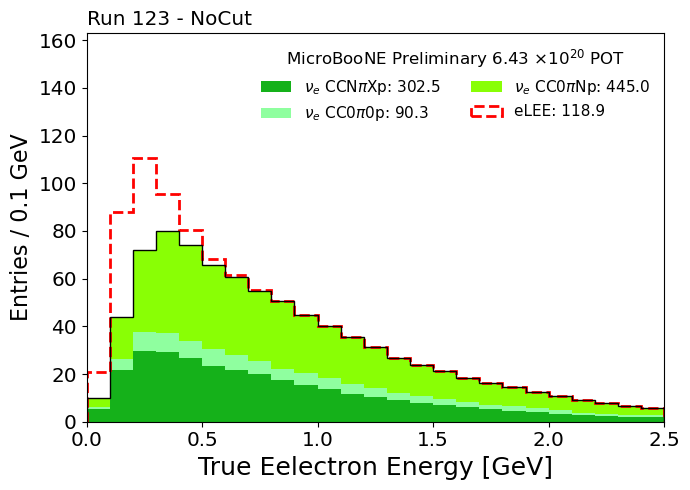
\includegraphics[width=\linewidth]{technote/SignalModel/Figures/old eLEE model shwKE.png}
        \caption{MicroBooNE electron energy spectrum in truth $\nu_e$ events.}
    \end{subfigure}    
    \begin{subfigure}{0.49\linewidth}
        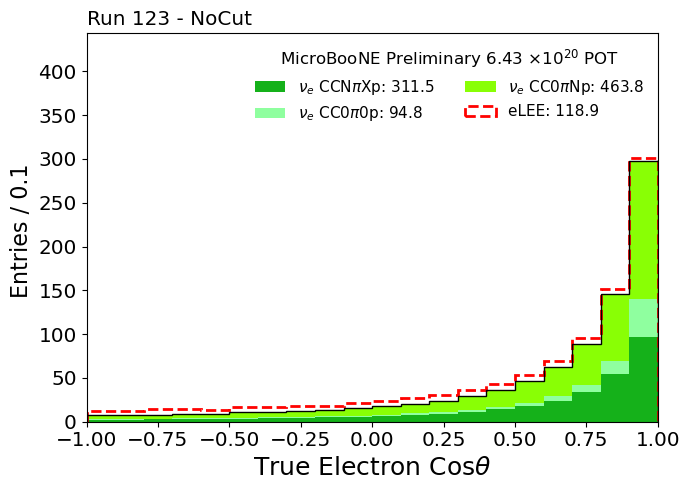
\includegraphics[width=\linewidth]{technote/SignalModel/Figures/old eLEE model shwAngle.png}
        \caption{MicroBooNE electron $\cos\theta$ spectrum in truth $\nu_e$ events.}
    \end{subfigure}
    \caption{The first eLEE model on MicroBooNE electron kinematics spectra in truth $\nu_e$ events before any selection cuts applied.}
    \label{fig:old_eLEE_truth}
\end{figure}

\subsection{Implementation}This model assumes that all the LEE events originate from intrinsic $\nu_e$ interactions in the flux, without relying on a specific underlying theoretical model. The excess in true electron 2D kinematic space (electron kinetic energy and $\cos\theta$) is obtained by unfolding the background-subtracted excess of data events in the reconstructed 2D shower kinematic space (shower energy and shower $\cos\theta$). This process utilizes MiniBooNE's selection efficiency and smearing matrix of final-state electrons. Fig. \ref{fig:MB_response} displays the response matrices for CCQE neutrino energy, shower energy, and shower $\cos\theta$, respectively. Unlike the excess model used in the previous PeLEE analysis, which unfolded the CCQE neutrino energy, this new signal model relies on final-state electrons, reducing CCQE modeling dependence.



The ratio between the predicted rate from MiniBooNE and that of the intrinsic electron neutrino component in MiniBooNE’s simulation is used to obtain a flux scaling factor for the excess under the electron neutrino hypothesis. The weights are applied to the rate of intrinsic electron neutrino events predicted by MicroBooNE’s flux and cross-section simulation to obtain a prediction for the MiniBooNE $\nu_e$-like excess in the MicroBooNE detector. The weights distributed in 2D electron kinematic space are shown in Fig.~\ref{fig:MB_ratio_b}. As a comparison, the energy-dependent weights from CCQE neutrino energy unfolding are shown in Fig.~\ref{fig:MB_ratio_a}.

Fig.~\ref{fig:uB_excess} shows MicroBooNE's truth-level electron energy and $\cos\theta$ spectra, broken into final-state topology. The signal model obtained from MiniBooNE dataset predicts visible excess mostly in the range of 150-500 MeV for electron energies , and 0.5-1.0 for electron $\cos\theta$.

\begin{figure}[H]
    \centering
    \begin{subfigure}{0.52\linewidth}
        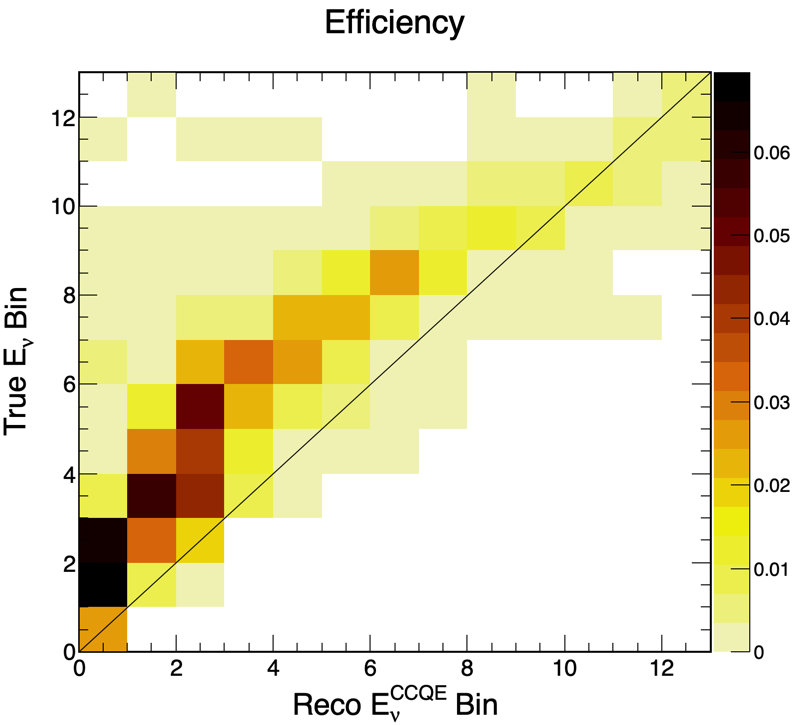
\includegraphics[width=\linewidth]{technote/SignalModel/Figures/NuE_RecoTrue_Eff_2D.png}
        \caption{MB CCQE neutrino energy.}
    \end{subfigure}
    \begin{subfigure}{0.49\linewidth}
        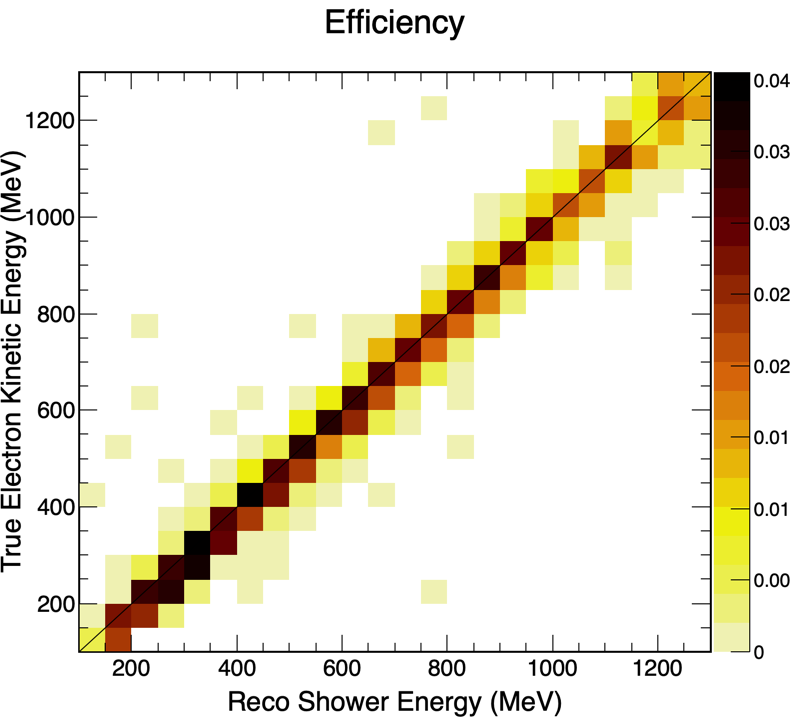
\includegraphics[width=\linewidth]{technote/SignalModel/Figures/ShwKE_RecoTrue_Eff_2D.png}
        \caption{MB shower energy.}
    \end{subfigure}    
    \begin{subfigure}{0.49\linewidth}
        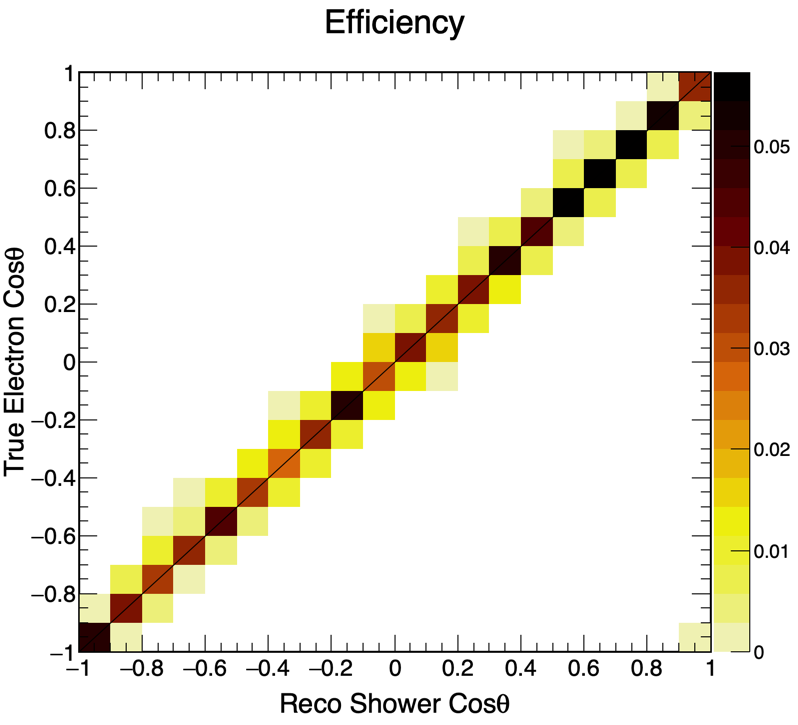
\includegraphics[width=\linewidth]{technote/SignalModel/Figures/ShwTheta_RecoTrue_Eff_2D.png}
        \caption{MB shower $\cos\theta$.}
    \end{subfigure}
    \caption{Semearing matrices for CCQE neutrino energy, shower energy and shower $\cos\theta$.}
    \label{fig:MB_response}
\end{figure}


\begin{figure}[H]
    \centering
    \begin{subfigure}{0.49\linewidth}
        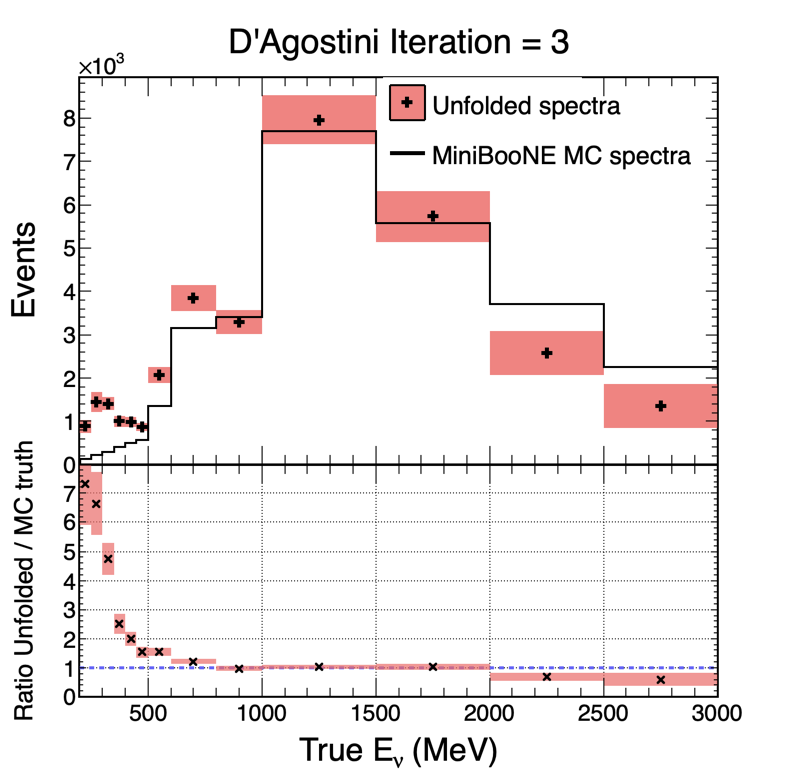
\includegraphics[width=\linewidth]{technote/SignalModel/Figures/NuE_model.png}
        \caption{MB CCQE neutrino energy.}\label{fig:MB_ratio_a}
    \end{subfigure}
    \begin{subfigure}{0.5\linewidth}
        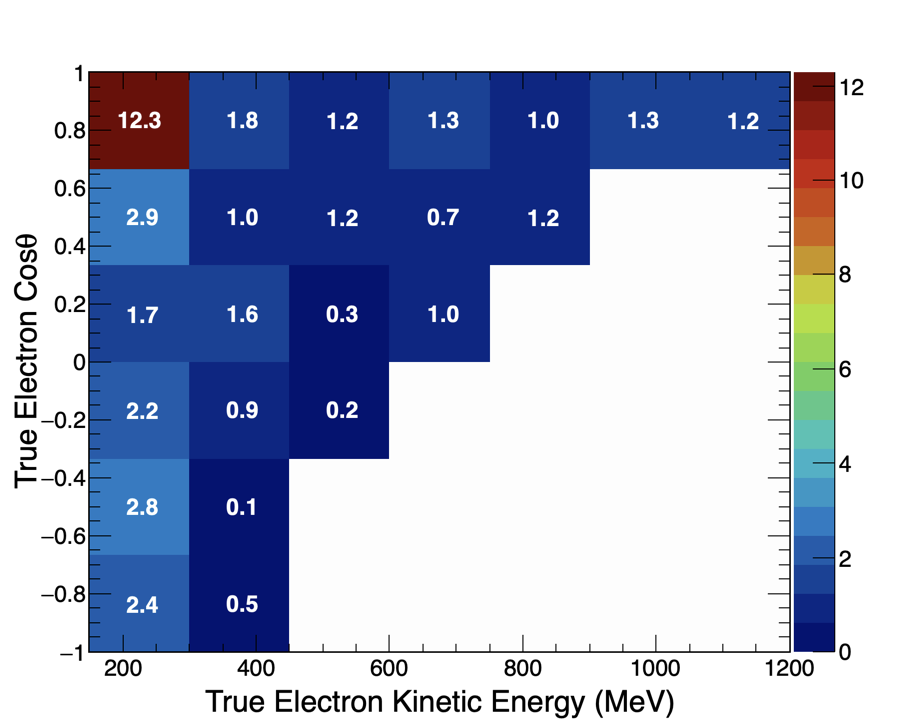
\includegraphics[width=\linewidth]{technote/SignalModel/Figures/Shw2D_model.png}
        \caption{MB shower 2D.}\label{fig:MB_ratio_b}
    \end{subfigure}
    \caption{MiniBooNE eLEE ratio models unfolded from CCQE neutrino energy and shower 2D kinematic variables.}
    \label{fig:MB_ratio}
\end{figure}

\begin{figure}[H]
    \centering
    \begin{subfigure}{0.49\linewidth}
        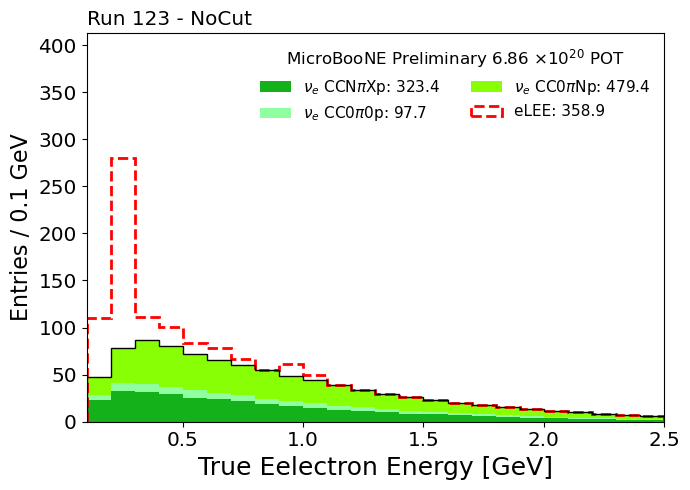
\includegraphics[width=\linewidth]{technote/SignalModel/Figures/uB_ShwKE_LEE.png}
        \caption{Electron energy.}
    \end{subfigure}
    \begin{subfigure}{0.49\linewidth}
        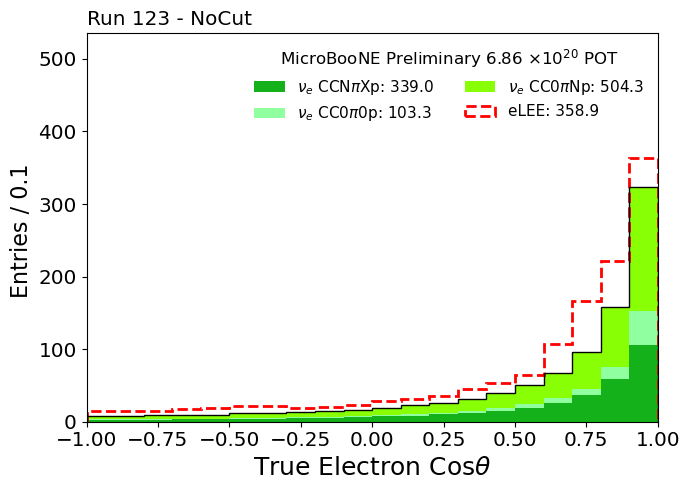
\includegraphics[width=\linewidth]{technote/SignalModel/Figures/uB_ShwTheta_LEE.png}
        \caption{Electron $\cos\theta$.}
    \end{subfigure}
    \caption{Excess model in MicroBooNE electron energy and $\cos\theta$.}
    \label{fig:uB_excess}
\end{figure}